\section{Syntaxes and Translation rules}
The precompiler takes SV+ in and outputs the Verilog RTL descriptions. So we defined the SV+ syntaxes and a subset of Verilog syntaxes that SV+ code being translated to. In this section, we give BNF definition of the main syntaxes and  translation rules the precompiler based on.
%%%%%%%%%%%%%%%%%%%%%%%%%%%%%%%%%%%%%%%%%%%%%%%%%%%%%%%%%%%%%%%%%%%%%%%%%%%%%%%%%%%%%%%%%%%%%%%%%
%\subsection{Compiling process}
%A typical cuicuit consists of two parts, the Datapath and Controller.
%\begin{figure}[h]
%\centering
%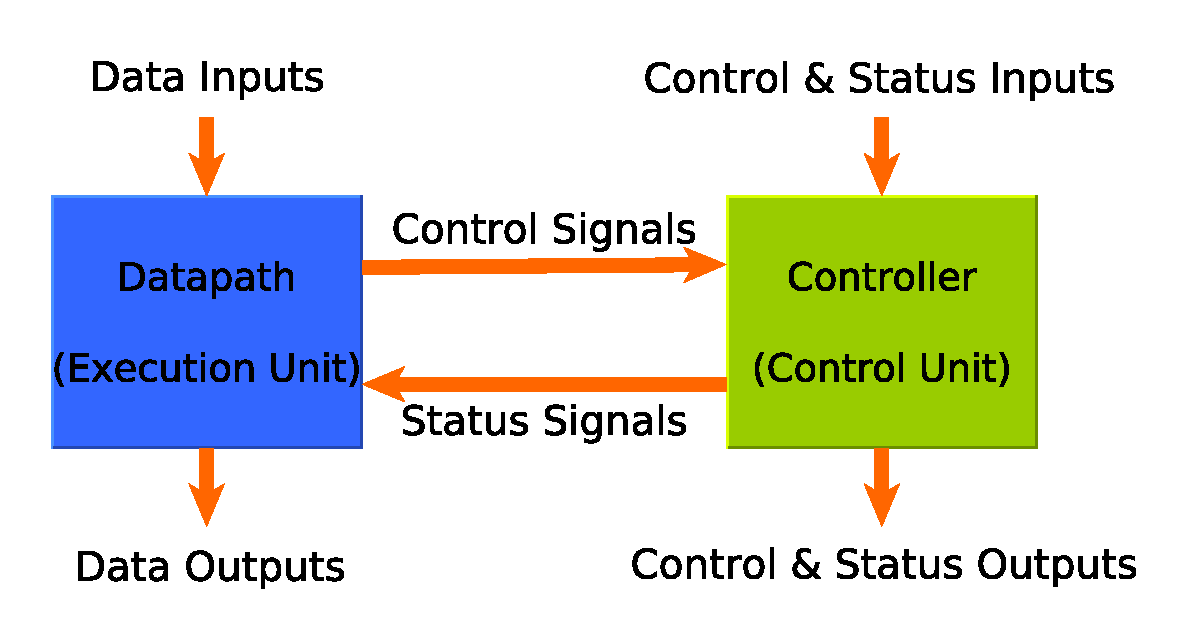
\includegraphics[scale=.4]{circuitstructure}
%\caption{The Circuit Structure}
%\label{fig-structure}
%\end{figure}
%Data flys into the datapath and get processed by datapath unit under the control of control singlas (usually %generated by a state machine) from the controller.\newline
%Our compiler takes both the datapath and controller despciptions, written with extended Verilog.
%%%%%%%%%%%%%%%%%%%%%%%%%%%%%%%%%%%%%%%%%%%%%%%%%%%%%%%%%%%%%%%%%%%%%%%%%%%%%%%%%%%%%%%%%%%%%%%%%%%
\subsubsection{SV+ Syntaxes}
SV+ is an embedded language which makes good use of the Verilog syntaxes. Only a small set of new syntaes are needed:
\itshape
\begin{enumerate}\itemsep2pt \parskip0pt \parsep0pt
  \item sv+ ::= fold | map | forloop
  \item fold ::= FOLD; id; id; id; id$^n$
  \item map ::= MAP; id; id; id; num; num
  \item forloop ::= FOR; id; fstatement$^n$
  \item fstatement ::= id; id*; id*
  \item id ::= signal | sum | var | moduleName | in
               | out | dataName
  \item num ::= h | l | datalen | maplen
  \item signal ::= string
  \item sum ::= string
  \item var ::= string
  \item moduleName ::= string
  \item in ::=  string
  \item out ::= string
  \item dataName ::= string
  \item h ::= integer
  \item l ::= integer
  \item datalen ::= integer
  \item maplen ::= integer
  \item MAP ::= "map"
  \item FOLD ::= "fold"
  \item FOR ::= "for"
\end{enumerate}
\normalfont
Though, $moduleName$, $input$, $output$, $sum$, $var$ are $id_s$, they take different postions in $fold$, $map$ and $forloop$, for simplicity the parser just identifies the statments and then gets values through relative order.\\
Notes on syntaxes:
%\itshape
\begin{itemize}\itemsep2pt \parskip0pt \parsep0pt
  \item[$\star$]\textit{1}: There are three new structures.
  \item[$\star$]\textit{2}: FOLD is keyword, then $id(signal)$, $id(sum)$, $id(var)$, $id^n(variables)$.
  \item[$\star$]\textit{3}: MAP is keyword, then $id(signal)$, $id(moduleName)$, $id(dataName)$, $num(datalen)$,
                            $num(maplen)$.
  \item[$\star$]\textit{4}: FOR is keyword, then id(signal), fstatements.
  \item[$\star$]\textit{5}: Statement in a forloop is a module with its ports, eg. $ADD(in0, in1, out)$.
  \item[$\star$]\textit{8,9,10,11,12,13,14}: These are just strings.
  \item[$\star$]\textit{15,16,17,18}: $h$, $l$, $datalen$, $maplen$ are numbers.
  \item[$\star$]\textit{19,20,21}: Keywords to indentify the new syntaxes.
\end{itemize}
%%%%%%%%%%%%%%%%%%%%%%%%%%%%%%%%%%%%%%%%%%%%%%%%%%%%%%%%%%%%%%%%%%%%%%%%%%%%%%%%%%%%%%%%%%%%%%%%%%%%%%%%%
\subsubsection{Verilog Syntaxes}
\normalfont
We defined structures $assign$, $operation$, $counter$ and $instance$ based on the basic Verilog elements. They are the essential bolcks which the SV+ circuit structure been mapped to. Usually, for example, a $map$ may be translated into a set of $counters$, $operations$, $instances$ and $assigns$. $Wires$, $regs$...are used to connect these Verilog structures if necessary.
\itshape
\begin{enumerate}\itemsep2pt \parskip0pt \parsep0pt
  \item verilogs ::= port | wire | reg | input | output |
                     oper | simpleassign | assign |
                     counter | instance
  \item wire ::= vid; vnum; vnum | vid
  \item reg ::= vid; vnum; vnum | vid
  \item input ::= vid; vnum; vnum | vid
  \item output ::= vid; vnum; vnum | vid
  \item oper :: id; reg; wire | id; reg; reg
  \item simpleassign ::= wire; reg
  \item assign ::= wire; reg; reg*
  \item counter ::= reg; vnum
  \item instance ::= vmoduleName; vinstanceName; vin*; vout*
  \item vid ::= vsignal | lvalue | rvalue | vin
                | vout | creg | vmoduleName
                | vinstanceName | vregName | vwireName
                | vinputName | voutputName
  \item vin ::= wire
  \item vout ::= reg
  \item ifc ::= reg; integer
  \item vnum ::= vh | vl
  \item port ::= string
  \item vsignal ::= string
  \item lvalue ::= string
  \item rvalue ::= string
  \item vmoduleName ::= string
  \item vinstanceName ::= string
  \item vh ::= integer
  \item vl ::= integer
  \item upbound ::= integer
\end{enumerate}
\normalfont
Notes:
\begin{itemize}\itemsep2pt \parskip0pt \parsep0pt
   \item[$\star$]\textit{1}: Verilog syntaxes subset.
   \item[$\star$]\textit{2,3,4,5}: Declarations or instances of resources in Verilog.
   \item[$\star$]\textit{6}: An always block in verilog, which contains an assignment, eg. $x[7{:}0] {<=} y[7{:}0]$.
   \item[$\star$]\textit{7}: eg. $assign\; x[7{:}0] {=} y[7{:}0]$.
   \item[$\star$]\textit{8}: A multiplexer, eg. $assign x {=} (g{==}0)?y:w$.
   \item[$\star$]\textit{9}: A register increases per cycle, makes zero at upbound.
   \item[$\star$]\textit{10}: Instantiation of sub-module.
   \item[$\star$]\textit{14}: If condition, eg. $if(r{==}1)$.
   \item[$\star$]\textit{16,17,18,19,20,21}: Treated as strings.
   \item[$\star$]\textit{22,23,24}: $vh$, $vl$ and $upbound$ are numbers.
\end{itemize}
%%%%%%%%%%%%%%%%%%%%%%%%%%%%%%%%%%%%%%%%%%%%%%%%%%%%%%%%%%%%%%%%%%%%%%%%%%%%%%%%%%%%%%%%%%%%%%%%%%%%%%%%%
\subsubsection{Translation rules}
\normalfont
Around one hundred rules were explored to translate SV+ descriptions into Verilog descriptions. For the demonstration purpose we just put those rules related with translating $map$ structure here and explain how they are used.
%\KZ{A rule can only have one conclusion. It can have multiple premises.
%Several rules below have more than one conclusion predicates! Also
%I don't know the meaning of these rules at all. And I think many of them
%are not correct!  Plus, give explanation of each rule.}
%********************************************
\[ \begin{aligned}
  \mathit{1.\;\frac{}{reg(regName, h, l)}}\;\;\;
  \mathit{2.\;\frac{}{wire(wireName, h, l)}}
\end{aligned}
\phantom{\hspace{100cm}}
\]
%%%
\[ \begin{aligned}
  \mathit{3.\;\frac{}{string(x) + string(y) \rightarrow string(x\_y)}}
\end{aligned}
\phantom{\hspace{100cm}}
\]
%%%
\[ \begin{aligned}
  \mathit{4.\;\frac{}{signal \rightarrow vsignal}}\;\;\;
  \mathit{5.\;\frac{signal \rightarrow vsignal}{id(signal) \rightarrow vid(vsignal)}}
\end{aligned}
\phantom{\hspace{100cm}}
\]
%%%
\[ \begin{aligned}
  \mathit{6.\;\frac{}{moduleName + string(i) \rightarrow vinstanceName}}\;\;\;
\end{aligned}
\phantom{\hspace{100cm}}
\]
%%%
\[ \begin{aligned}
  \mathit{7.\;\frac{moduleName \rightarrow vmoduleName}{id(moduleName) \rightarrow vid(vmoduleName)}}\;\;\;
\end{aligned}
\phantom{\hspace{100cm}}
\]
%%%
%\[ \begin{aligned}
%  \mathit{9.\;\frac{}{h \rightarrow vh}}\;\;\;
%  \mathit{10.\;\frac{h \rightarrow vh}{num(h) \rightarrow vnum(vh)}}\;\;\;
%\end{aligned}
%\phantom{\hspace{100cm}}
%\]
%%%
\[ \begin{aligned}
  \mathit{8.\;\frac{}{l \rightarrow vl}}\;\;\;
  \mathit{9.\;\frac{l \rightarrow vl}{num(l) \rightarrow vnum(vl)}}\;\;\;
\end{aligned}
\phantom{\hspace{100cm}}
\]
%%%
\[ \begin{aligned}
  \mathit{10.\;\frac{}{dataName \rightarrow regName}}\;\;\;
\end{aligned}
\phantom{\hspace{100cm}}
\]
%%%
\[ \begin{aligned}
  \mathit{11.\;\frac{dataName \rightarrow regName}{id(dataName) \rightarrow vid(regName)}}\;\;\;
\end{aligned}
\phantom{\hspace{100cm}}
\]
%%%
\[ \begin{aligned}
  \mathit{n=u{/}d,}\\
  \mathit{reg(m\_c,d{-}1,0),}\\
  \mathit{wire(m\_in,d{-}1,0),}  \\
  \mathit{wire(m\_out,d{-}1,0),}\\
  \mathit{signal(s) \rightarrow vsignal(s)}\\
  \mathit{dataName(r) \rightarrow regName(r),}\\
  \mathit{moduleName(m) \rightarrow vmoduleName(m),}\\
  \mathit{moduleName(m){+}1 \rightarrow vinstanceName(m\_1),}\\
  \mathit{12.\;\frac{}{map(MAP; id(s),id(m),id(r),num(u),num(d)) \rightarrow}}\\
  \mathit{counter(m\_c,n),}\\
  \mathit{assign(m\_in, m\_c, reg_n(r,u{-}1,u{-}d),...,}\\
  \mathit{reg_1(r,d{-}1,0)),} \\
  \mathit{instance(m,m\_1,m\_in,m\_out),}\\
  \mathit{oper_1(s \&\& ifcon(m\_c,1),reg(r,u{-}1,u{-}d),m\_out),}\\
  \mathit{\cdots}\\
  \mathit{oper_n(s \&\& ifcon(m\_c,n),reg(r,u{-}1,u{-}d),m\_out)}
\end{aligned}
\phantom{\hspace{100cm}}
\]
%%%
\[ \begin{aligned}
  \mathit{n=u{/}d,}\\
  \mathit{wire(m\_in,u{-}1,0),}\\
  \mathit{wire(m\_out,u{-}1,0),}\\
  \mathit{signal(s) \rightarrow vsignal(s)} \\
  \mathit{dataName(r) \rightarrow regName(r),}\\
  \mathit{moduleName(m) \rightarrow vmoduleName(m),}\\
  \mathit{moduleName(m){+}n \rightarrow vinstanceName(m\_n),}\\
  \mathit{\cdots}\\
  \mathit{moduleName(m){+}1 \rightarrow vinstanceName(m\_1),}\\
  \mathit{13.\;\frac{}{map(MAP; id(s),id(m),id(r),num(u),num(d)) \rightarrow}}\\
  \mathit{simpleassign(m\_in,r),oper(s,r,m\_out),}\\
  \mathit{instance_n(m,m\_n,wire(m\_in,u{-}1,u{-}d),}\\
  \mathit{wire(m\_out,u{-}1,u{-}d)),}\\
  \mathit{\cdots}\\
  \mathit{instance_1(m,m\_n,wire(m\_in,d{-}1,0),}\\
  \mathit{wire(m\_out,d{-}1,0))}\\
\end{aligned}
\phantom{\hspace{100cm}}
\]
%%%
\normalfont
Rule notes:
\begin{itemize}\itemsep2pt \parskip0pt \parsep0pt
  \item[$\star$]\textit{1,2}: Declaration or instance of \textit{reg, wire}.
  \item[$\star$]\textit{3}: String concatenation.
  \item[$\star$]\textit{6}: Nameing rule to name a module's instance.
  \item[$\star$]\textit{12}: In this rule that used to translate a map structure we used only
                 one sub-module instance Data u bits flows into this sub-
                 module in  n cycles and d bits per cycle. A counter which generates m\_c
                 used in assign and opers controls the in-out order. N opers
                 bolocks put the outputs from the sub-module into data list, under control
                 of map's singal and the counter.
  \item[$\star$]\textit{13}: In this rule we used $n=u/b$
                 sub-module instances So we can get each d-bit of the data processed
                 parallelly.Two u-bits width wires defined to connect the data with n
                 sub-module instances. When $vsignal(s)$ is active, data gets refreshed
                 in block $oper$.
\end{itemize}
\section{More Examples}
Four examples have been discussed in this section. To demo the usage of our proposed syntax in real design and show that the pre-compiler makes work easier and sometimes more interesting, since the programmer can use one statement to express the computation meaning of the circuit structure and gain diverse implementations after compiling it. Among the examples, there are simple ones, like SCM\cite{SCM} and widely used circuits such as DCT and FFT, as well as a more complex circuit, the AES\cite{AES}.
\subsection{Single Constant Multiplication(SCM)}
\subsubsection{What is SCM}
A multiplication by a fixed-point constant can be done "multiplierless" using addtions (or subtractions) and shifts only. As a simple example,
\begin{math}
y = 5x
\end{math}
can be computed as
\begin{equation}
y = (x<<2) + x
\end{equation}
Such a solution is called a multiplier block.\\
A straightforward way of multiplying by a given constant c using add/subtracts and shifts only can be read from c. We call it the binary method. For example,
\begin{math}
y = 45x
\end{math}
can be expressed as (since 45 = 00101101):
\begin{equation}
y = (x<<5) + (x<<3) + (x<<2) + (x)
\label{eq:scm}
\end{equation}
\subsubsection{Implementation of SCM}
We can use the $fold$ statments to describe equation\eqref{eq:scm}. The embedded SV+ code is:
\begin{verbatim}
always@(posedge clk)
if(fold_i)
begin
   fold(sum, var, 5, 3, 2, 0);
end
\end{verbatim}
%A sequential circuit will be generated
Basically, a combinatorial circuit that calculates expression\eqref{eq:scm} consists of three adders and three shifters, and some connection wires. However, for a sequential circuit, we can make trade-offs bwtween adder/shifter resource and performance.

\subsection{Fast Fourier Transform (FFT)}
%
\subsubsection{Fourier Series}
Any periodic waveform can be decomposed into a series of \begin{math} \sin \end{math} and \begin{math} \cos \end{math} waves. The general expression is showed below,
\begin{equation}
g(t) = \sum_{n=0}^\infty A_n\cos (\frac{2\pi nt}{T}) + \sum_{n=0}^\infty B_n\sin (\frac{2\pi nt}{T})
\end{equation}
The Fourier Transform is a methmatical operation which converts time-domain signals to the frequency domain.
%
%
\subsubsection{Discrete Fourier Transform}
Discrete Fourier Transform(DFT) is a version of Fourier Transform that can be applied to sampled time-domain signals. The DFT produces a discrete frequency spectrum, i.e. amplitude levels at discrete frequencies. The DFT is defined as:
\begin{equation}
X(k) = \sum_{n=0}^{N-1}x(n)e^{\frac{-j2\pi kn}{N}}\;\;\;\; 0\leq k \leq N-1
\end{equation}
Where, \begin{math} N \end{math} is the total number of samples taken from the original signal. Each signal in the transformed sequence $X(k)$ depends on every input signal $x(n)$.
%
%
\subsubsection{Fast Fourier Transform}
Computing the DFT of n samples directly according fomular "ref" requires \begin{math} O(n) \end{math} operations. However, this can be reduced to \begin{math} O(n\log n) \end{math} using well-know fast algorithms(Fast Fourier Transforms or FFTs), such as the Cooley-Tukey algorithm\cite{Cooley-TukeyAlgorithm}.
%
%
\subsubsection{Implementation of FFT}
%
Two main components are needed to implement FFT circuits. The first is a $butterfly \; circuit$, which takes inputs $x_0$ and $x_1$ to two outputs $x_0 + x_1$ and $x_0 - x_1$ (see figure \ref{fig-butterfly}). It is the heart of FFT implementations since it computes the 2-point DFT. Systems of such components will be applied to the in-signals in many stages (figure \ref{fig-2radixfft}, in this example there are 3 stages).\\
\begin{figure}[h]
\centering
\epsfig{file=butterfly.eps,width=0.4\columnwidth}
%\includegraphics[scale=1]{butterfly}
\caption{The Butterfly Operation}
\label{fig-butterfly}
\end{figure}
\begin{figure}[h]
\centering
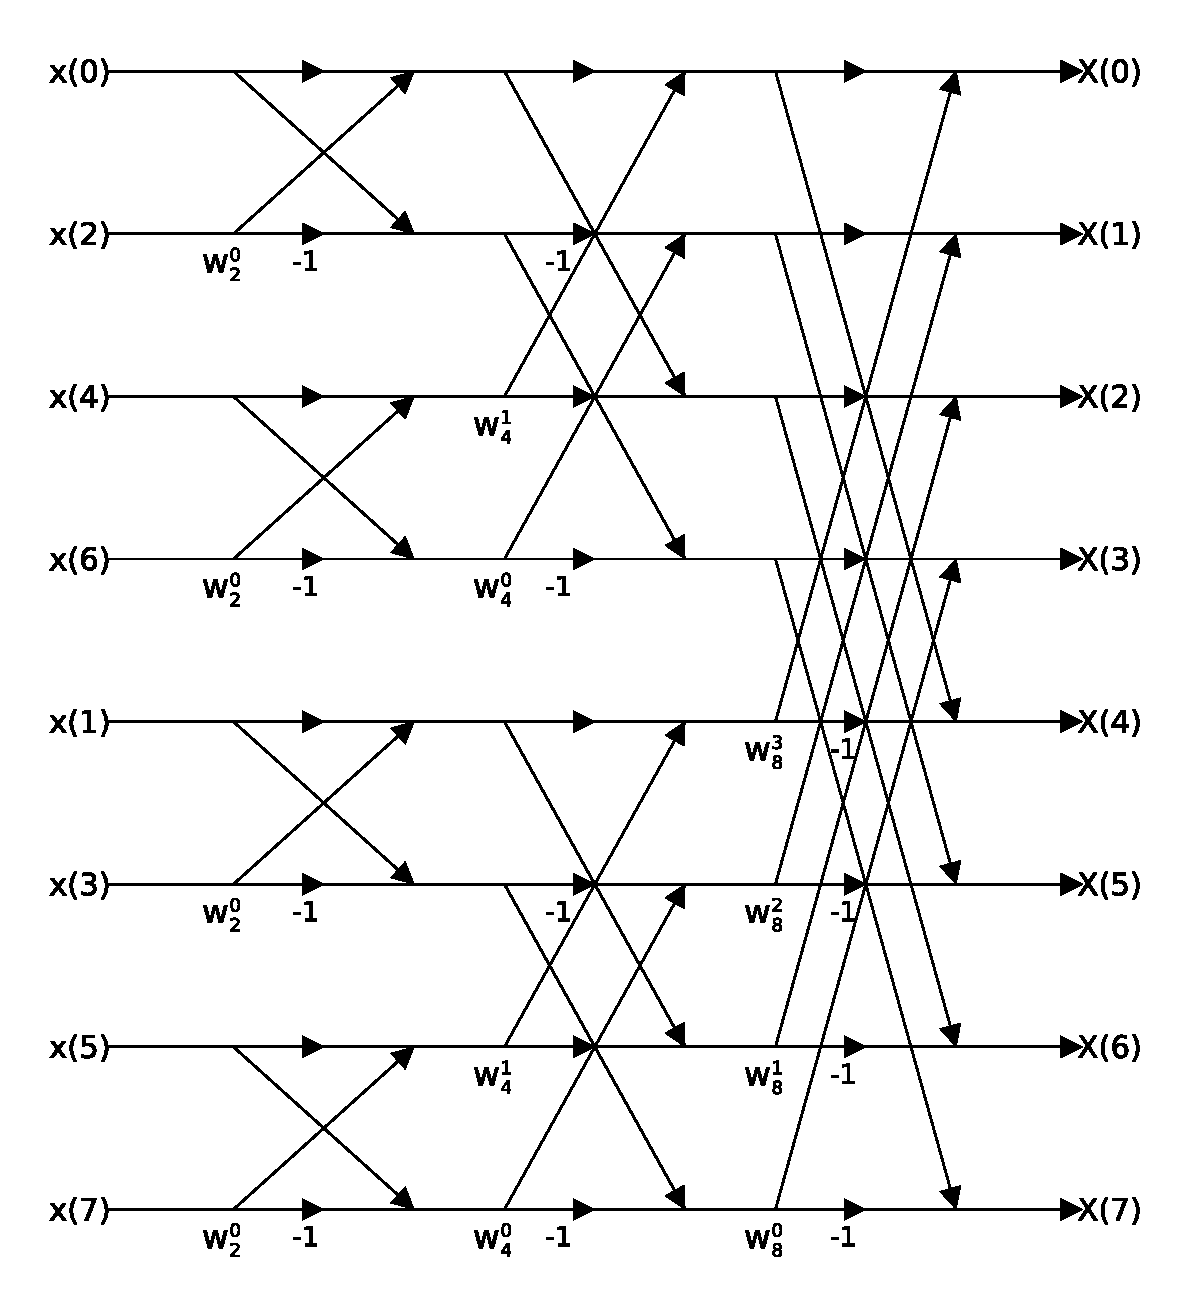
\epsfig{file=2radixfft,width=0.5\columnwidth}
%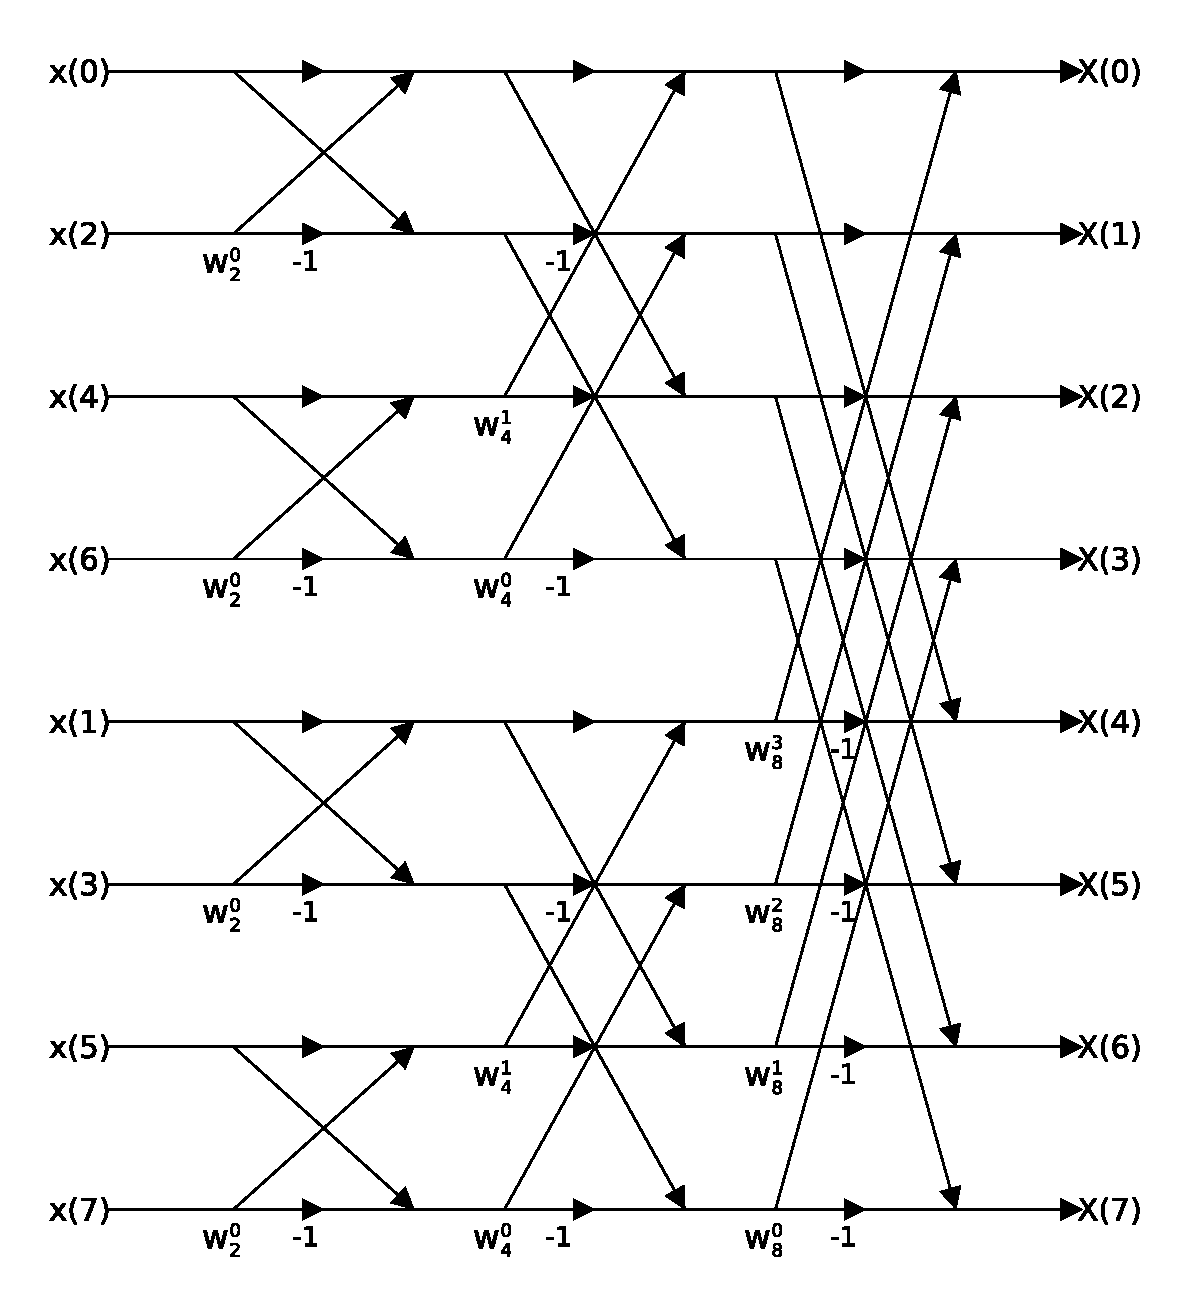
\includegraphics[scale=0.7]{2radixfft}
\caption{Dataflow for 8-Point Radix 2 FFT}
\label{fig-2radixfft}
\end{figure}
Another important component of an FFT algorithm is multiplication by a complex constant $W_N^k$, called a twiddle factor multiplier. In this implementation, we write these two components as a basic module.
\[ module\;\; butterfly(x_0, x_1, w, y_0, y_1);\]
and then invok this module in three forloops.
\begin{verbatim}
STAGE 1:
alway @(posedge clk)
if(f1_i)
  for
    butterfly(x0,x2,w,y0,y1);
    butterfly(x4,x6,w,y2,y3);
    butterfly(x1,x3,w,y4,y5);
    butterfly(x5,x7,w,y6,y7);
  end
\end{verbatim}
\begin{verbatim}
STAGE 2:
alway @(posedge clk)
if(f1_i)
  for
    butterfly(x0,x2,w,y0,y1);
    butterfly(x4,x6,w,y2,y3);
    butterfly(x1,x3,w,y4,y5);
    butterfly(x5,x7,w,y6,y7);
  end
\end{verbatim}
\begin{verbatim}
STAGE 3:
    ...
\end{verbatim}

\subsection{Discrete Consine Transform}
\subsubsection{What is Discrete Consine Transform}
This important transform (DCT for short) was first described by Alhmed at [] and has been used and studied extensively since, Syed Ali discussed it's thoery and application in details in []. Here we just give a brief introduction to DCT in one dimetiona, defined by:
%\begin{math}
\[  X_{k} = \sum_{n=0}^{N-1}x_{n}\cos[\frac{\pi}{N}(n+\frac{1}{2})k],\;\;\;k = 0,...,N\!\!-\!\!1 \]
%\end{math}
The N real numbers \begin{math}x_{0},...,x_{N-1}\end{math} are transformed into the N real numbers \begin{math}X_{0},...,X_{N-1}\end{math} arroding to formula above.
\subsubsection{Implementation of DCT}
In this implementation, we first compute the coefficents of DCT by:
\[
G_{f} = \sqrt{\frac{2}{N}}C_{f}\sum_{t=0}^{N-1}p_{t}\cos[\frac{(2t+1)f\pi}{2n}],f = 0,...,N\!\!-\!\!1
\]
where \[ C_{f} \left\{ \begin{array}{ll}
\frac{1}{\sqrt{2}}, & f = 0, \\ 1, & f > 0.
\end{array}
\right.
\]
Then we have:
\[ \left[
\begin{array}{llll}
X_{0} \\ X_{2} \\ X_{4} \\ X_{6}
\end{array}
 \right] = \left[ \begin{array}{cccc}
 a & a & a & a \\ a & f & -f & -c \\ a & -a & -a & a \\ f & -c & c & -f
 \end{array}
 \right] \left[ \begin{array}{llll}
 x(0)+x(7) \\ x(1)+x(6) \\ x(2)+x(5) \\ x(3)+x(4)
 \end{array}
 \right]
\]
\[ \left[
\begin{array}{llll}
X_{1} \\ X_{3} \\ X_{5} \\ X_{7}
\end{array}
 \right] = \left[ \begin{array}{cccc}
 b & d & e & g \\ d & -g & -b & -e \\ e & -b & g & d \\ g & -e & d & -b
 \end{array}
 \right] \left[ \begin{array}{llll}
 x(0)-x(7) \\ x(1)-x(6) \\ x(2)-x(5) \\ x(3)-x(4)
 \end{array}
 \right]
\]
where \[ \left[ \begin{array}{lllllll}
a \\ b \\ c \\ d \\ e \\ f \\ g
\end{array}
\right]  = \sqrt{\frac{2}{N}} \left[ \begin{array}{lllllll}
\cos\frac{\pi}{4} \\ \cos\frac{\pi}{16} \\ \cos\frac{\pi}{8} \\
\cos\frac{3\pi}{16} \\ \cos\frac{5\pi}{16} \\ \cos\frac{3\pi}{8} \\
\cos\frac{7\pi}{16}
\end{array}
\right] = \left[ \begin{array}{lllllll}
0.35355339 \\ 0.49039264 \\ 0.46193976 \\ 0.41573480 \\
0.27778511 \\ 0.19134171 \\ 0.09754516
\end{array}
\right]
\]
The computation denoted by matrix multiply can be written in SV+ code with three forloop:
\begin{verbatim}
LOOP1:                |   LOOP2:
always@(posedge clk)  |   always@(posedge clk)
if(m1i)               |   if(m1i)
for                   |   for
  y0 = x0 + x7;       |     y1 = x0 - x7;
  y2 = x1 + x6;       |     y3 = x1 - x6;
  y4 = x2 + x5;       |     y5 = x2 - x5;
  y6 = x3 + x4;       |     y7 = x3 - x4;
end                   |   end
\end{verbatim}
\begin{verbatim}
LOOP3:
always@(posedge clk)
if(m2i)
for
   X0 = a*y0 + a*y2 + a*y4 + a*y6;
   X2 = a*y0 + f*y2 + (-f)*y4 + (-c)*y6;
   X4 = a*y0 + (-a)*y2 + (-a)*y[4] + a*y6;
   X6 = f*y0 + (-c)*y2 + c*y4 + (-f)*y6;
   X1 = b*y1 + d*y[3] + e*y[5] + g*y7;
   X3 = d*y1 + (-g)*y3 + (-b)*y5 + (-e)*y7;
   X5 = e*y1 + (-b)*y3 + g*y5 + d*y7;
   X7 = g*y1 + (-e)*y3 + d*y5 + (-b)*y7;
end
\end{verbatim}
The benefit of writting is, the operation is the same in the forloop body, thus we can configurations on the number of arithmetics units. For example, in LOOP1, we can use 1, 2 or 4 adder(s) to finish the addtions. Pay attention to one thing here, in LOOP1 and LOOP2 the control signals are the same, means that these tow forloops could cun parallel. What's more, we can code the forloops in different ways, such as combine LOOP1 and LOOP2:
\begin{verbatim}
always@(posedge clk)
if(m1i)
for
   y0 = x0 + x7;
   y2 = x1 + x6;
   y4 = x2 + x5;
   y6 = x3 + x4;
   y1 = x0 + (-x7);
   y3 = x1 + (-x6);
   y5 = x2 + (-x5);
   y7 = x3 + (-x4);
end
\end{verbatim}
so that, we can even use one adder to do the addtions and subtractions.
